\begin{figure}[h!]
\small
\begin{center}
\setlength{\tabcolsep}{1pt}
\begin{tabular}{ccc}

\hspace{3mm} Training PSD & 
\hspace{3mm} Reconstruction PSD & 
\hspace{3mm} PSD Score  \\

%\vspace{-2mm}
%%%%% ORCA025 %%%%%%%%

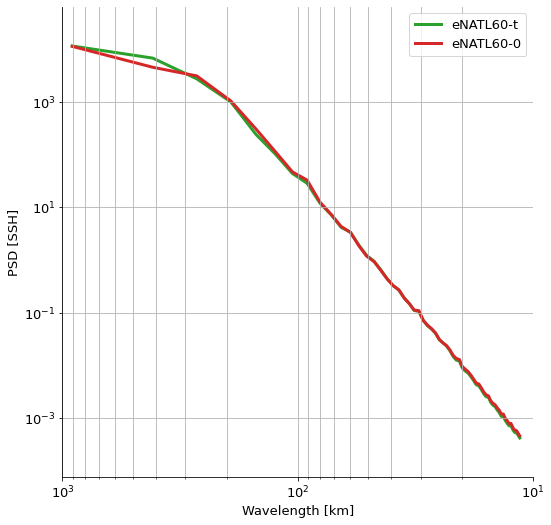
\includegraphics[width=0.32\textwidth]{figures/plots/isotrop_psd_tide_train.png} &
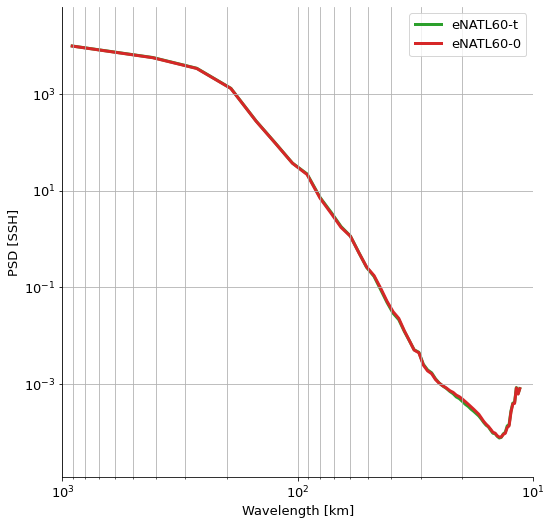
\includegraphics[width=0.32\textwidth]{figures/plots/isotrop_psd_tide_rec.png} &
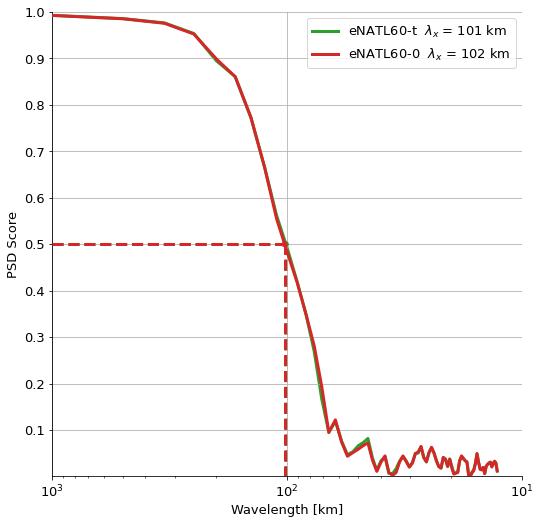
\includegraphics[width=0.32\textwidth]{figures/plots/tide_1d_psd_score.png}


\end{tabular}
\vspace{-3mm}
% \caption{Row I - Isotrophic PSD. Row 2 - Isotrophic PSD Score}
\caption{
Space-time spectral densities of the training datasets (first row) and their associated reconstructions}\vspace{-5mm}
\label{fig:res1}
\end{center}
\end{figure}
